\section{Experimental Design and Evidence}\label{sec:experiments}

\subsection{Experimental roadmap}\label{sec:exp-roadmap}
The experiments follow the argument developed in the theory.  E1 isolates the path-dependent reference mechanism and its decision consequence.  E2 evaluates the frozen-target gradient estimator in the shared semi-synthetic setup.  E3 releases the same setup as a continuous slow-variation process and tests online first-order tracking, while E4 maps the robustness of that tracking result over reference, horizon, and optimizer perturbations.  E5 then moves to a time-ordered real A-share replay under common trading constraints.  E6 holds real investor decisions, controls, chronological split, and predictive model fixed while changing only the reference representation.  E7 replays the E5 recommendations through investor types calibrated from E6 and historical behavior, separating recommendation adoption from satisfaction after adoption.  \Cref{fig:evidence-map} summarizes the theory-aligned core and these three external-validity layers.

\begin{figure}[t]
    \centering
    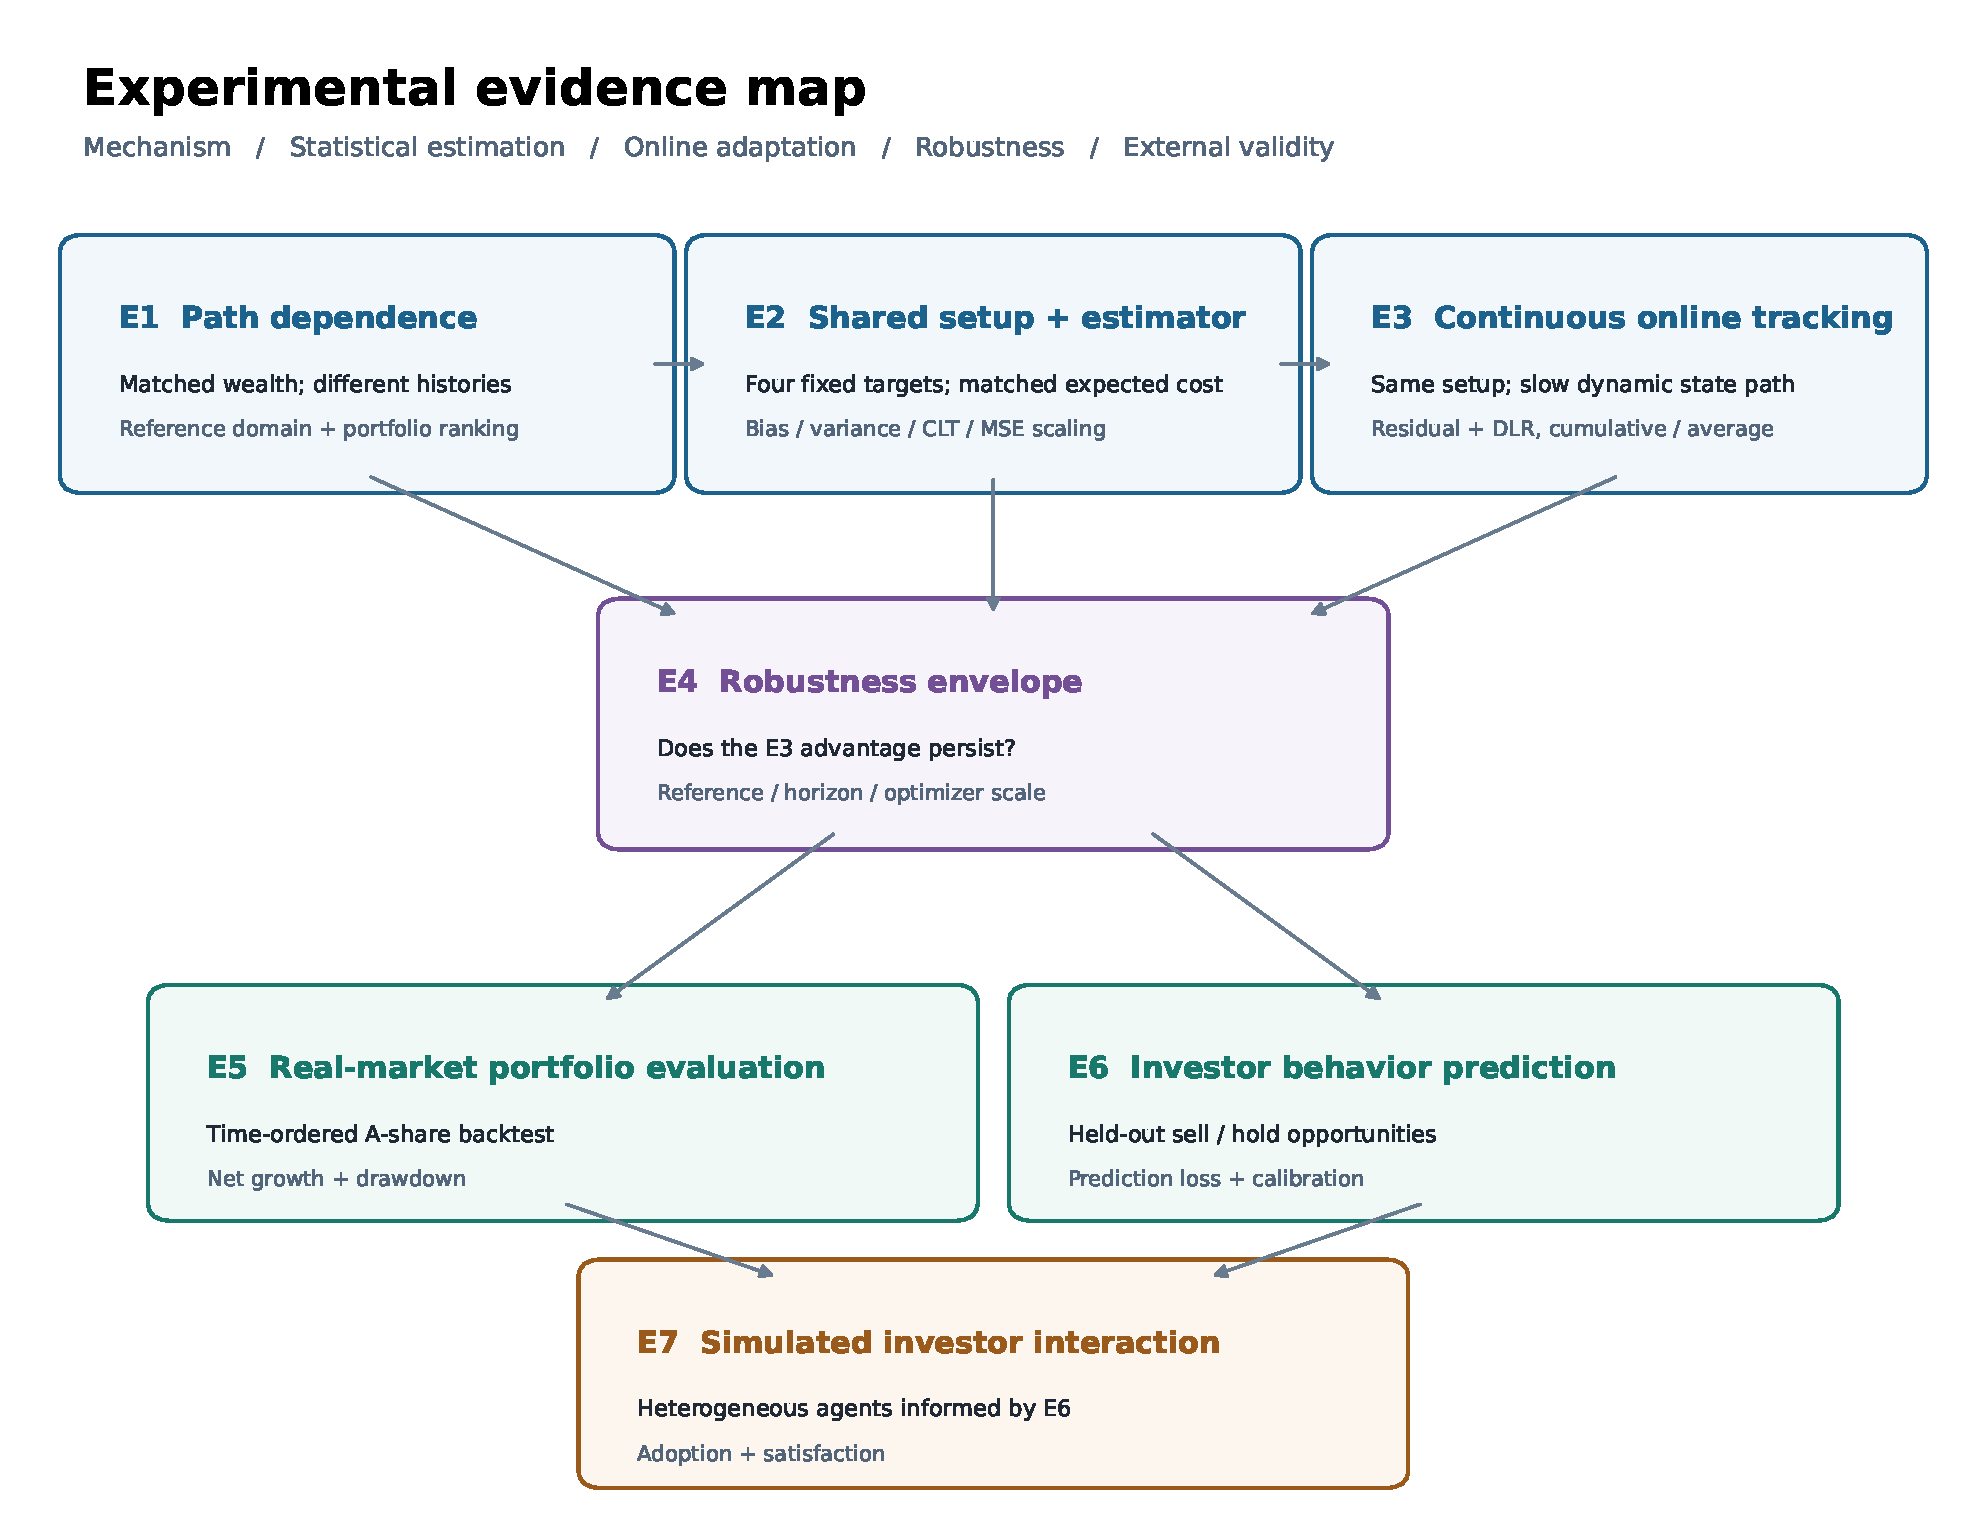
\includegraphics[width=0.96\textwidth]{figures/experiment_evidence_map.pdf}
    \caption{Experimental evidence map for the theory-aligned core.  E1 establishes the decision consequence of path-dependent reference formation; E2 evaluates the frozen-target gradient estimator; E3 measures continuous first-order tracking; and E4 maps robustness.  E5--E7 follow this core as external-validity layers for market, behavior, and interaction, while keeping their estimands separate from the E2--E4 statistical and tracking diagnostics.}
    \label{fig:evidence-map}
\end{figure}
\FloatBarrier

\subsection{E1: Path dependence and portfolio choice}\label{sec:e1}
\paragraph{Design.}
We construct two histories with the same initial wealth and the same endpoint,
\[
(1,1.10,1.015)
\qquad\text{and}\qquad
(1,0.90,1.015),
\]
and apply the reference recursion in \eqref{eq:reference-update} with $(\eta_+,\eta_-)=(0.20,0.05)$.  The histories are matched at the decision time: current wealth is $X_T=1.015$, the pre-trade portfolio is $50\%$ cash and $50\%$ risky asset, and the next risky return is $+4\%$ with probability $p$ and $-4\%$ otherwise.  We compare two feasible target allocations, $20\%$ and $80\%$ risky.  Under the action inertia in \eqref{eq:action-map}, these targets execute as $44\%$ and $56\%$ risky.  Because the next-period distribution has two states, all CPT values are evaluated exactly rather than by Monte Carlo.

\begin{figure}[t]
    \centering
    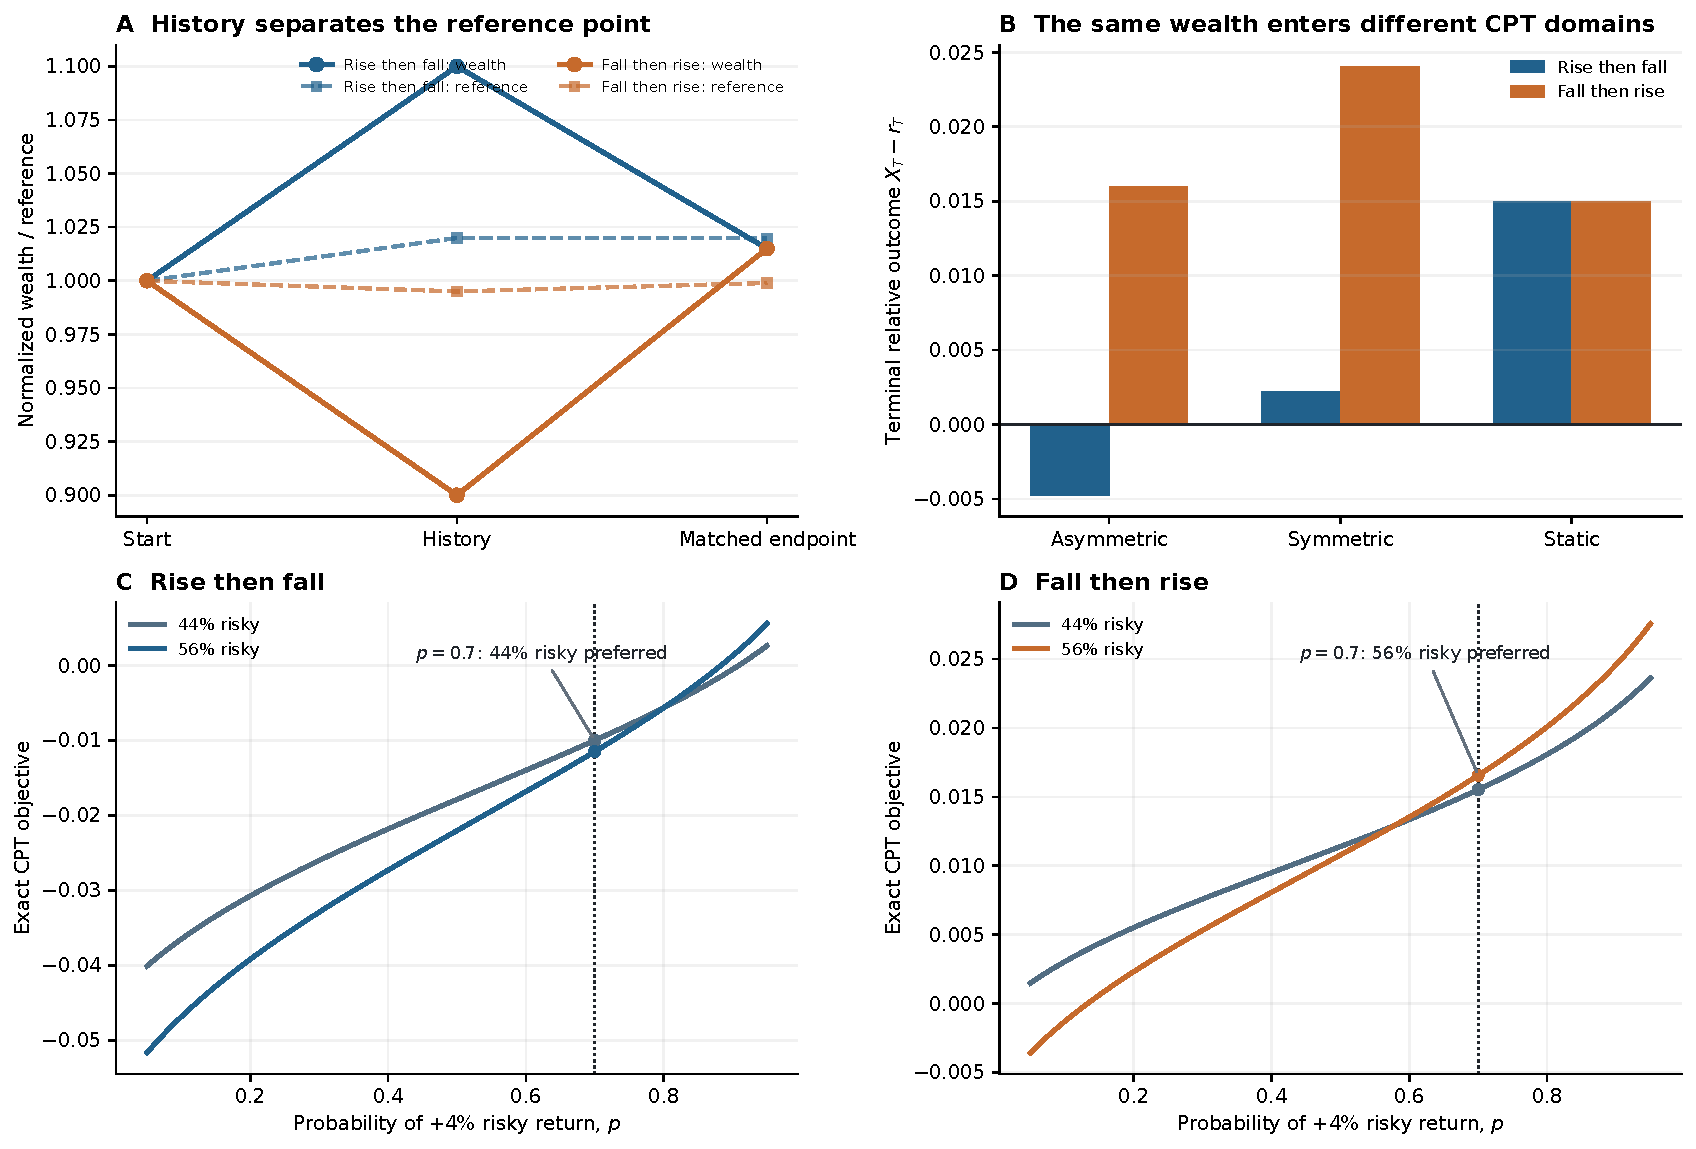
\includegraphics[width=\textwidth]{figures/e1_path_and_decision_final.pdf}
    \caption{Path dependence changes both the perceived domain and the portfolio ranking.  \textbf{A}: The two histories end at the same wealth but generate different asymmetric reference points.  \textbf{B}: The asymmetric rule places the rise--fall history below its reference and the fall--rise history above its reference; the symmetric and static rules provide mechanism controls.  \textbf{C--D}: Exact CPT values of the two feasible executed allocations as the probability $p$ of a $+4\%$ risky return varies.  At $p=0.7$, the matched rise--fall account prefers $44\%$ risky whereas the matched fall--rise account prefers $56\%$ risky.}
    \label{fig:e1-path-choice}
\end{figure}

\begin{table}[t]
\centering
\caption{E1 exact mechanism summary at $p=0.7$.}
\label{tab:e1-summary}
\begin{tabular}{lrrrrl}
\toprule
History & $X_T$ & $r_T$ & $X_T-r_T$ & Preferred risky share & CPT domain \\
\midrule
Rise then fall & 1.015 & 1.01975 & $-0.00475$ & 44\% & Loss \\
Fall then rise & 1.015 & 0.99900 & $+0.01600$ & 56\% & Gain \\
\bottomrule
\end{tabular}
\end{table}
\FloatBarrier

\paragraph{Results.}
The same terminal wealth is evaluated on opposite sides of the CPT reference.  After the rise--fall history, the reference is $1.01975$, so $X_T-r_T=-0.00475$; after the fall--rise history it is $0.999$, so $X_T-r_T=0.016$.  The separation propagates to the decision itself.  At $p=0.7$, the rise--fall history gives CPT values $-0.01001$ and $-0.01151$ for the $44\%$ and $56\%$ risky allocations, respectively, while the fall--rise history gives $0.01552$ and $0.01656$.  Thus two investors with identical current wealth, holdings, and opportunity set rank the same feasible portfolios differently solely because their histories imply different reference points.  This is the decision-level consequence of the path dependence characterized in \Cref{prop:path-dependence}.
\FloatBarrier

\subsection{E2: Finite-sample gradient estimation}\label{sec:e2}
\paragraph{Shared semi-synthetic setup.}
Beginning with E2, we use a common $30$-stock-plus-cash semi-synthetic market built from a frozen empirical A-share factor-block library.  Factor blocks are sampled from a time-invariant empirical distribution, while the return law follows a pre-specified path across episodes.  For risky asset $i$ in episode $k$,
\[
R_{i,k,u}=0.08\,\tanh\!\left(
\frac{\mu_k+2.5\,b_k^\top f_{i,u}+\xi^{\rm com}_{k,u}+\xi^{\rm id}_{i,k,u}}{0.08}
\right),
\]
where the common and idiosyncratic shocks have standard deviations $0.006s_k$ and $0.009s_k$, respectively.  Episodes $1$--$40$ use the stable momentum law, episodes $41$--$60$ use the reversal law, episodes $61$--$120$ interpolate to the terminal low-volatility/value/quality law, and the exogenous return law is fixed thereafter.  E2 standardizes the account context to
\[
(X,r,\omega,\theta)=(1,1,e_{\rm cash},0)
\]
and freezes four pre-specified targets at episodes $20$, $50$, $90$, and $150$, corresponding to the stable, post-change, mid-drift, and post-drift phases.  E3 subsequently uses the same factor distribution and episode-specific return law but allows the account state to evolve continuously.

We compare the proposed centered leave-one-out estimator with independent raw randomized correction against the raw independent-split plug-in estimator used by the adapted CPT-PG v5 baseline.  Both target the square-smoothed CPT objective in \eqref{eq:value-functions}.  Expected complete-trajectory cost is matched over
\[
\mathsf B\in\{32,64,128,256,512,1024,2048\},
\]
and numerical gradient references are generated independently at substantially higher cost.

\begin{figure}[t]
    \centering
    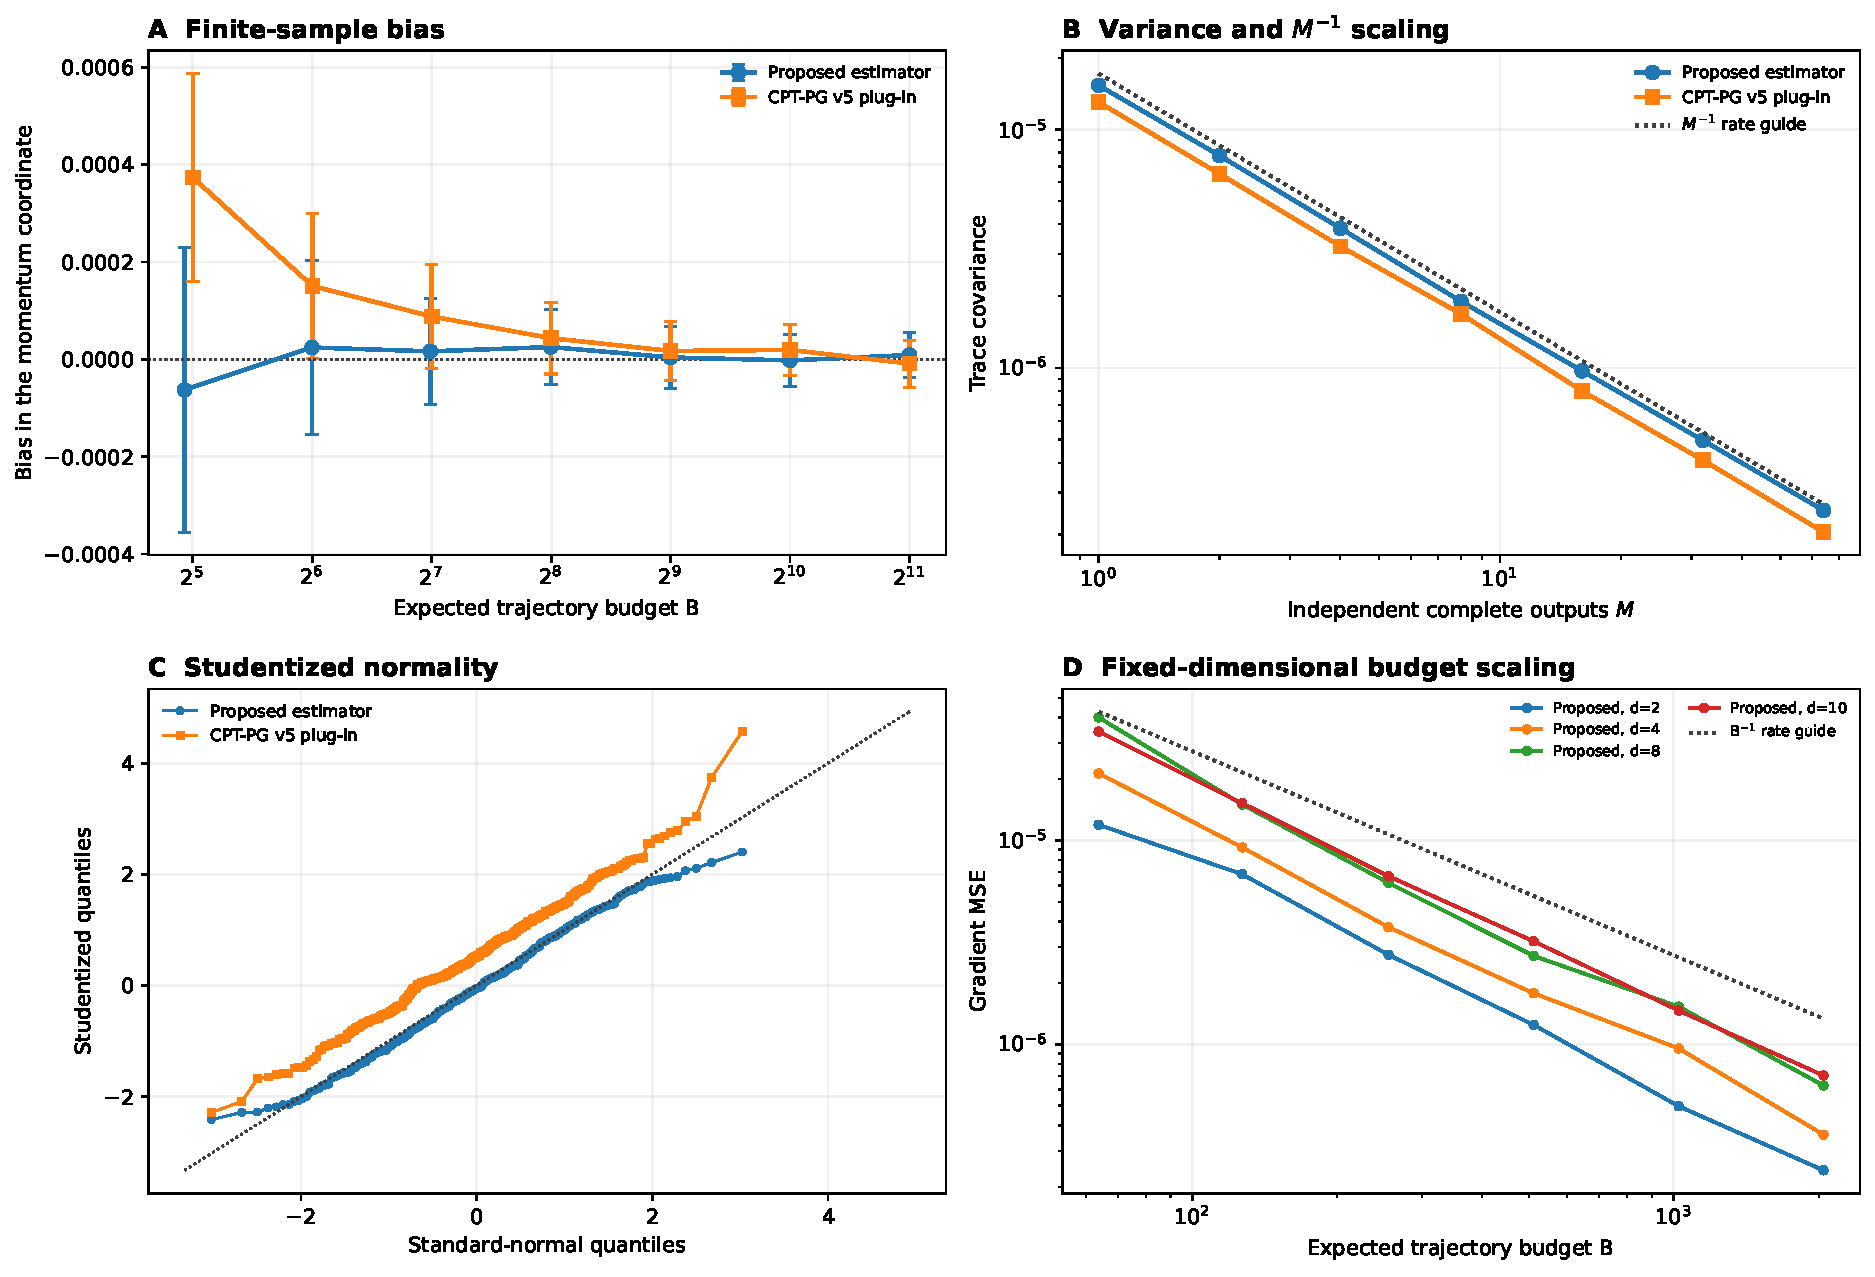
\includegraphics[width=\textwidth]{figures/e2_estimator_diagnostics.pdf}
    \caption{Finite-sample gradient estimation in the shared semi-synthetic setup.  \textbf{A}: coordinate bias at the stable target.  \textbf{B}: trace covariance of averages of $M$ independent complete estimator outputs; the dotted reference has slope $-1$.  \textbf{C}: studentized normal-quantile diagnostic at $M=64$.  \textbf{D}: full-gradient MSE versus expected trajectory budget for $d\in\{2,4,8,10\}$; the dotted reference has slope $-1$.  The corresponding unbiasedness, asymptotic normality, and fixed-dimensional minimax statements are given in \Cref{thm:estimator,thm:clt,thm:minimax}.}
    \label{fig:e2-estimator}
\end{figure}

\begin{table}[t]
\centering
\small
\caption{Full-gradient MSE at expected trajectory budget $\mathsf B=512$ across the four fixed targets.  MSE entries are in units of $10^{-6}$.  The last column gives a paired 95\% bootstrap interval for $\mathrm{MSE}_{\rm prop}-\mathrm{MSE}_{\rm v5}$ in the same units.}
\label{tab:e2-period-mse}
\begin{tabular}{lrrrr}
\toprule
Target & Proposed & CPT-PG v5 & Ratio & Difference 95\% CI \\
\midrule
Stable & 3.123 & 2.938 & 1.063 & $[-0.055,\ 0.434]$ \\
Post-change & 10.134 & 10.809 & 0.938 & $[-1.495,\ 0.139]$ \\
Mid-drift & 10.647 & 11.468 & 0.928 & $[-1.739,\ 0.102]$ \\
Post-drift & 10.589 & 12.257 & 0.864 & $[-2.599,-0.721]$ \\
\bottomrule
\end{tabular}
\end{table}
\FloatBarrier

\paragraph{Results.}
The four diagnostics separate estimator centering from ordinary Monte Carlo variance.  At the stable target, the proposed coordinate estimate remains centered near the numerical reference across the budget range, while the plug-in estimator exhibits the larger low-budget displacement expected from nonlinear probability weighting (\Cref{fig:e2-estimator}A).  Once independent complete outputs are averaged, both estimators recover the predicted inverse-replication variance rate: the fitted log--log slopes are $-0.989$ for the proposed estimator and $-0.999$ for CPT-PG v5 (\Cref{fig:e2-estimator}B).  The proposed estimator also exhibits inverse-budget full-gradient MSE across $d=2,4,8,10$, with slopes between $-1.17$ and $-1.12$, consistent with the fixed-dimensional $\Theta(\mathsf B^{-1})$ rate in \Cref{thm:minimax}.

The studentized outputs sharpen the centering comparison.  At $M=64$, the proposed statistic has mean $-0.049$, standard deviation $0.993$, and 95\% coverage of $96.25\%$, whereas the v5 statistic has mean $0.556$ and coverage of $91.75\%$ (\Cref{fig:e2-estimator}C).  At the standard budget $\mathsf B=512$, the proposed estimator has the lower MSE point estimate in three of the four fixed targets; the post-drift reduction is $13.6\%$ and its paired interval lies entirely below zero (\Cref{tab:e2-period-mse}).  Thus the debiased construction preserves the expected $1/\mathsf B$ statistical rate while improving finite-sample centering and delivering competitive or lower full-gradient error across the pre-specified market states.
\FloatBarrier

\subsection{E3: Continuous slow-variation online tracking}\label{sec:e3}
\paragraph{Design.}
E3 releases the market setup introduced in E2 as one continuous online process.  No account state is reset.  If a five-day episode starting from $(X_k,r_k,\omega_k)$ produces the raw terminal state $(\widetilde X_{k+1},\widetilde r_{k+1},\widetilde\omega_{k+1})$, the next episode starts from the diminishing-gain transition
\[
\begin{aligned}
\log X_{k+1}
&=(1-\alpha_k)\log X_k+\alpha_k\log\widetilde X_{k+1},\\
r_{k+1}
&=(1-\alpha_k)r_k+\alpha_k\widetilde r_{k+1},\\
\omega_{k+1}
&=(1-\alpha_k)\omega_k+\alpha_k\widetilde\omega_{k+1},
\qquad
\alpha_k=k^{-3/4}.
\end{aligned}
\]
The within-episode reference update remains the asymmetric mechanism in \eqref{eq:reference-update} with $(\eta_+,\eta_-)=(0.20,0.05)$.  Hence the reference point retains its cross-episode memory, while bounded raw transitions imply episode-start state increments of order $O(\alpha_k)$ and
\[
\sum_{k\le K}\alpha_k=O(K^{1/4})=o(K).
\]
The factor-block distribution is time invariant, the exogenous return coefficients follow the E2 phase path through episode $120$, and remain fixed for episodes $121$--$300$.  This construction keeps the dynamic-reference system continuous while imposing a sublinear state-step budget, providing the theory-aligned slow-variation setting used to probe \Cref{cor:vanishing-tracking}.

The comparison uses $20$ independent test trajectories.  The online learner and frozen control share the complete path through episode $40$.  Thereafter the online learner continues Algorithm~\ref{alg:drcptpg}, whereas the control freezes $\theta$ but continues to propagate wealth, reference, and holdings under the same slow transition.  We fix $(\gamma,\vartheta)=(0.08,0.05)$ before the E3 test runs and use the growing replication schedule
\[
M_k=\max\{4,\lceil\sqrt{k}\rceil\},
\]
so that the average inverse replication count decays as $O(K^{-1/2})$ by \eqref{eq:growing-replication-bound}.  DLR follows \eqref{eq:dynamic-regret} with $w=5$ and $\rho=0.9$.  Two independent evaluation streams estimate both the squared projected residual and the squared norm of the window-averaged projected residual by cross-stream products, preventing the ordinary self-square noise term from entering the evaluation.

\begin{figure}[t]
    \centering
    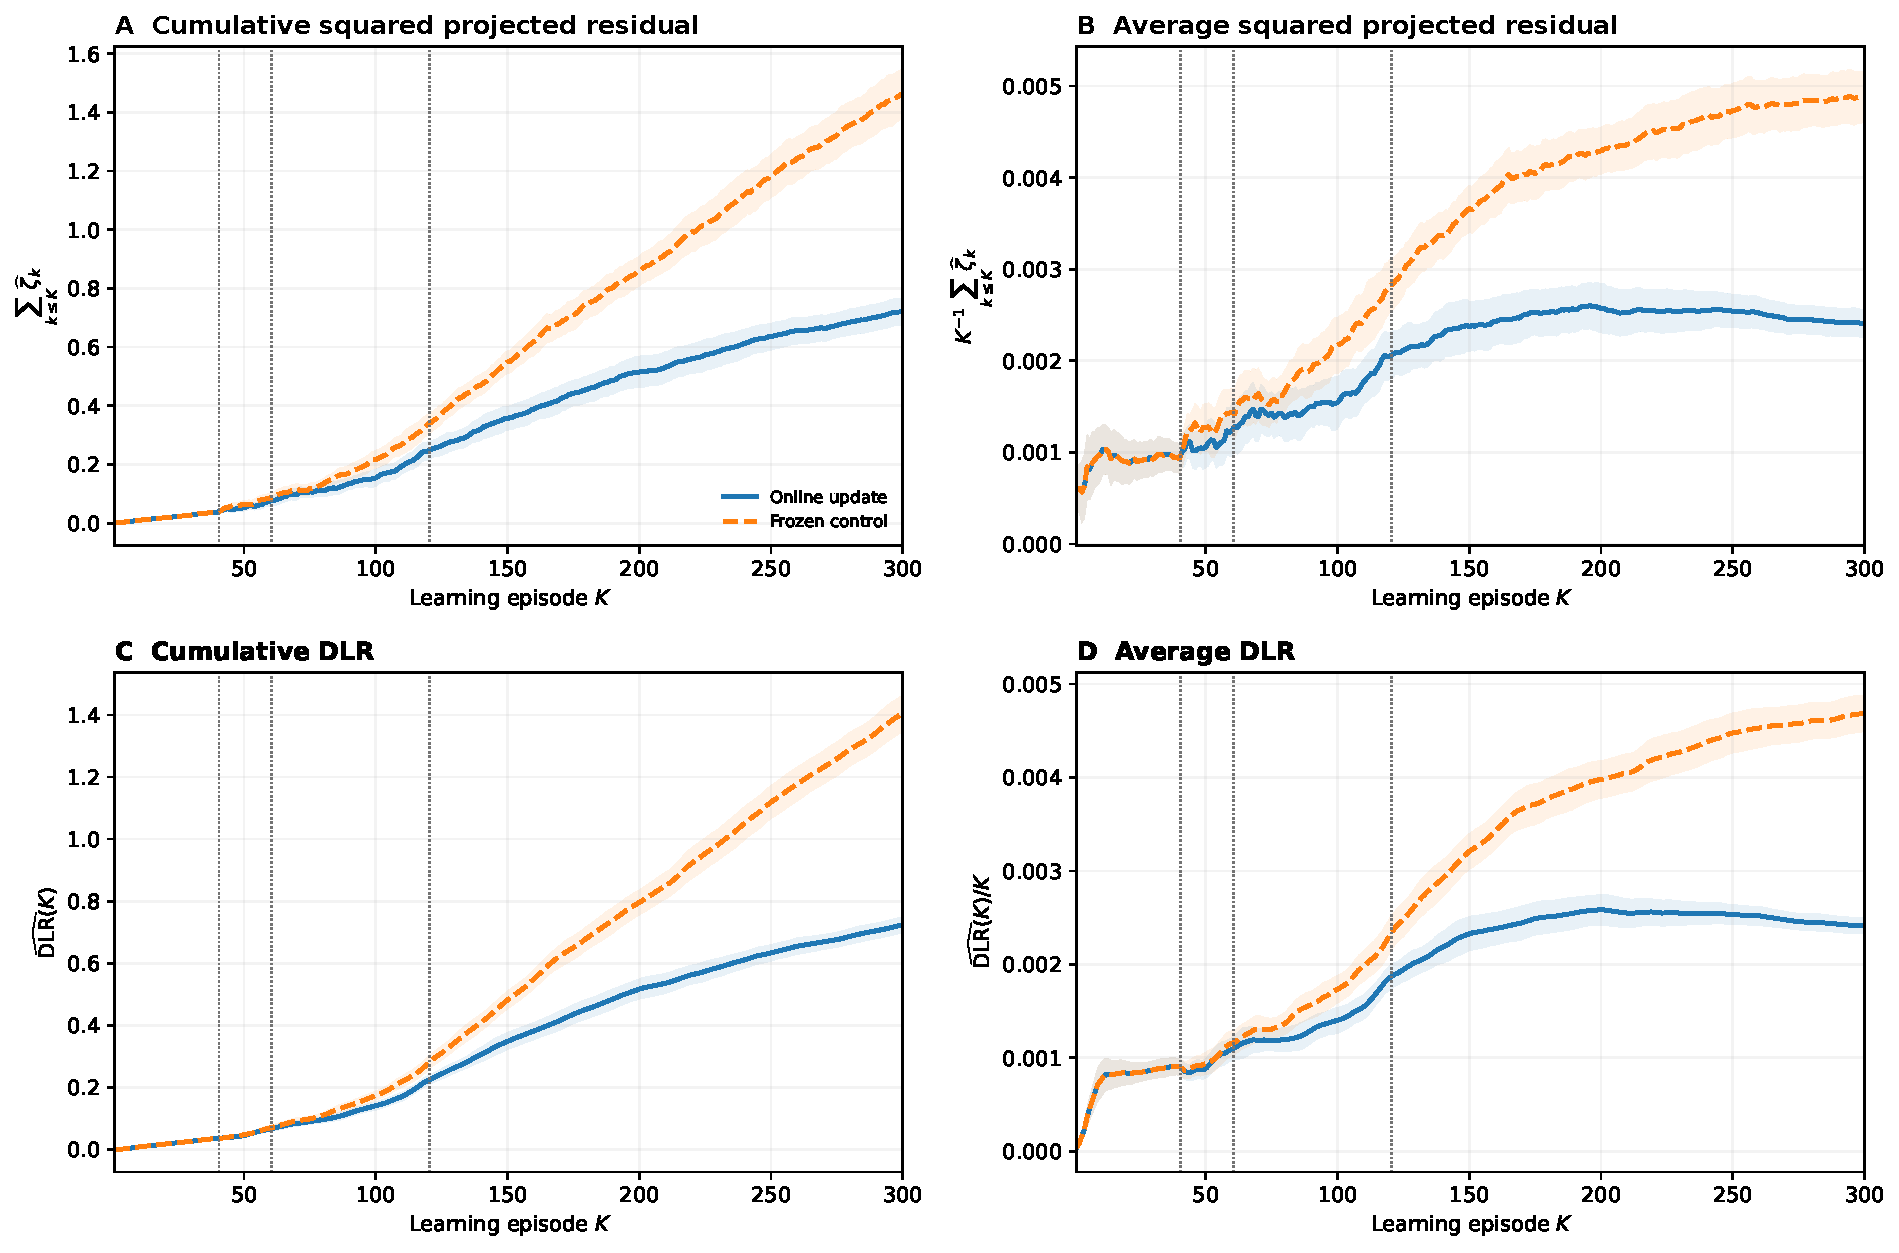
\includegraphics[width=\textwidth]{figures/e3_online_tracking.pdf}
    \caption{Continuous online tracking under slow variation.  \textbf{A--B}: cumulative squared projected residual and its average.  \textbf{C--D}: cumulative and average DLR.  The two methods share the same trajectory through episode $40$; thereafter the frozen control holds $\theta$ fixed while both methods continue to propagate their own wealth, reference, and holdings.  Dotted lines mark the abrupt change, the start of gradual drift, and the point after which the exogenous return law is fixed.  Curves are means over $20$ independent trajectories and shaded bands are $1.96$ standard errors.}
    \label{fig:e3-tracking}
\end{figure}
\FloatBarrier

\paragraph{Results.}
Continued updating produces substantially lower closed-loop tracking accumulation than freezing the policy parameter after episode $40$.  Over episodes $41$--$300$, cumulative squared projected residual is $0.684$ for the online learner and $1.427$ for the frozen control, while cumulative DLR is $0.687$ versus $1.369$; the seed-paired differences have 95\% bootstrap intervals $[-0.834,-0.650]$ and $[-0.738,-0.622]$, respectively.  By episode $300$, average DLR is $2.411\times10^{-3}$ online and $4.685\times10^{-3}$ frozen (\Cref{fig:e3-tracking}D).  Because the policies induce different endogenous account paths after they diverge, the frozen curve is a closed-loop control rather than a common-objective optimizer comparison.  The direct theory-aligned diagnostic is therefore the evolution of the squared projected residual and DLR along its own moving objective sequence.

The slow-variation tail also changes the growth rate of accumulated tracking error.  Over episodes $121$--$300$, the empirical log--log slope of cumulative DLR is $0.704$ for continued updating and $0.968$ for the frozen control; the corresponding cumulative squared projected residual slopes are $0.745$ and $0.959$.  The online exponent below one is consistent with the sublinear direction predicted by \Cref{cor:dynamic-local-regret,cor:vanishing-tracking} for a slowly varying target sequence.  Under the optional error-bound condition in \Cref{ass:error-bound}, the average expected squared projected residual also controls the average squared distance from its policy iterates to the contemporaneous stationary set through \Cref{cor:stationary-tracking}.
\FloatBarrier

\subsection{E4: Robustness of online tracking}\label{sec:e4}
\paragraph{Design.}
E4 tests whether the E3 closed-loop tracking advantage persists when the reference dynamics, decision horizon, and optimizer scale are perturbed.  Because each perturbation changes the induced objective sequence, absolute DLR values are not compared across configurations.  Instead, within each configuration $c$ we report the matched-control ratio
\[
\mathcal R_{\rm DLR}(c)
=\frac{\mathrm{DLR}^{\rm post}_{\rm online}(c)}{\mathrm{DLR}^{\rm post}_{\rm frozen}(c)},
\]
where the post-change interval begins at the first regime change.  This is a within-configuration normalization of the same DLR used in E3, not a new loss; $\mathcal R_{\rm DLR}<1$ means that continued updating accumulates less DLR than freezing $\theta$ under the same configuration.

Panel A evaluates the full $9\times9$ reference grid
\[
\eta_+,\eta_-\in\{0,0.05,0.10,\ldots,0.40\}.
\]
Panel B varies the episode horizon over
\[
h\in\{1,2,4,5,10,20,25,50\},
\]
while holding total market time at $1500$ days and tying the state-gain clock to elapsed market time.  Panel C evaluates $48$ admissible optimizer configurations from
\[
\gamma\in\{0.01,0.02,0.03,0.04,0.05,0.06,0.08,0.10,0.12\},
\]
\[
\vartheta\in\{0.005,0.01,0.015,0.02,0.03,0.04,0.05,0.06\},
\qquad
\gamma L_{\rm diag}\le\vartheta,
\quad L_{\rm diag}=0.31.
\]
The E3 defaults $(\eta_+,\eta_-)=(0.20,0.05)$, $h=5$, and $(\gamma,\vartheta)=(0.08,0.05)$ are marked but are not re-selected in E4.  Each configuration uses four independent paired trajectories.

\begin{figure}[H]
    \centering
    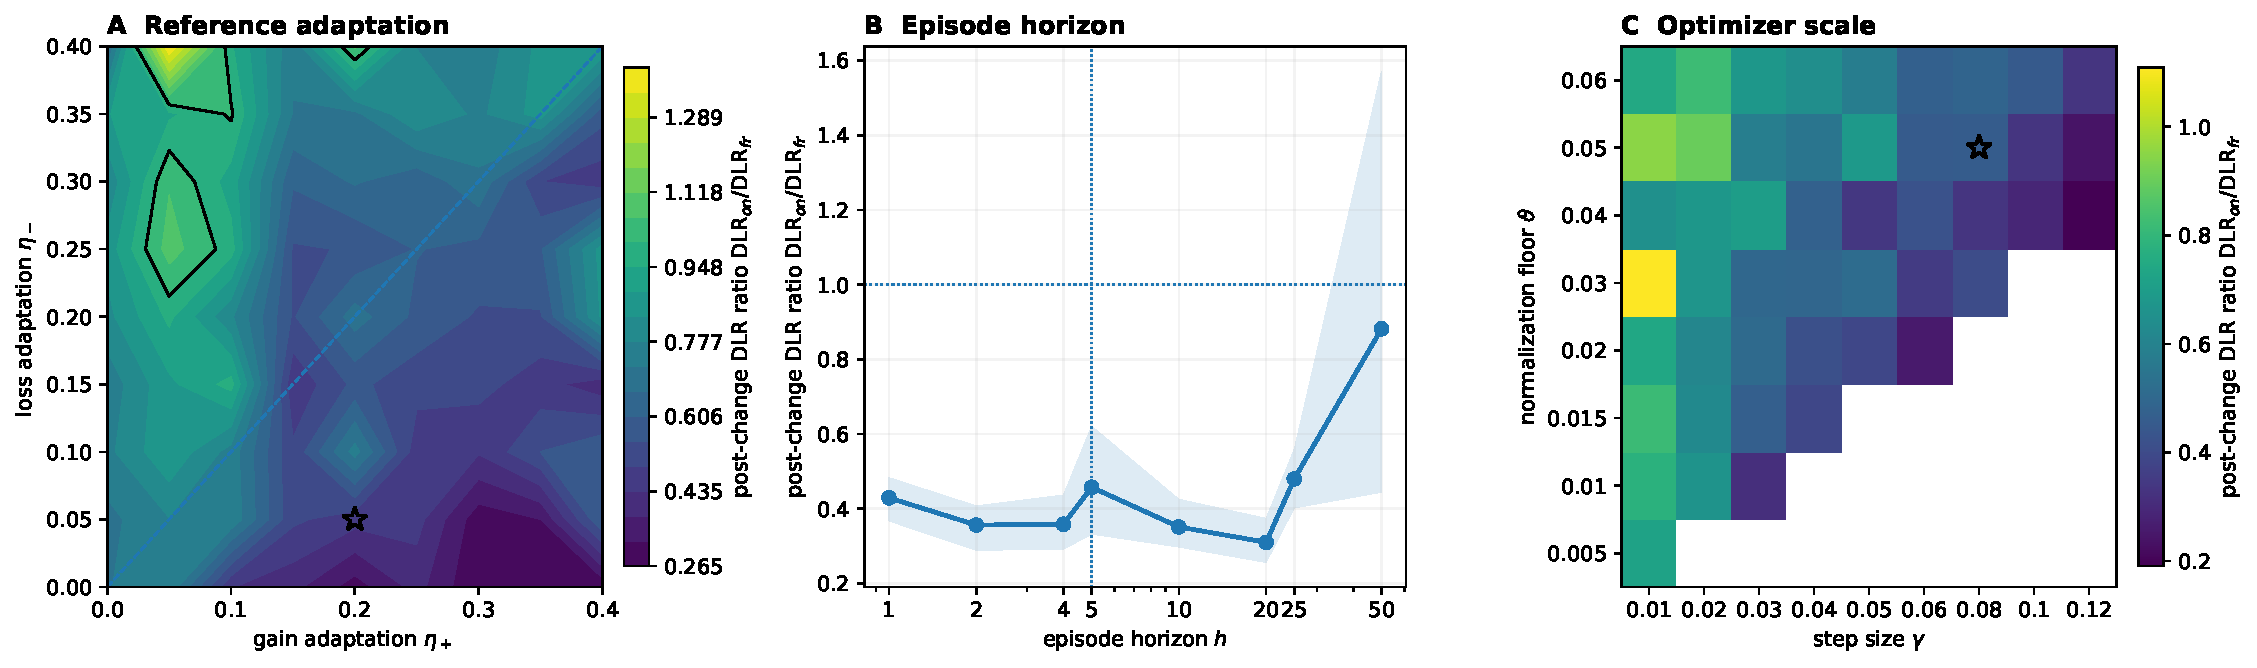
\includegraphics[width=\textwidth]{figures/e4_robustness.pdf}
    \caption{Robustness of the online-tracking advantage measured by the configuration-matched post-change DLR ratio $\mathcal R_{\rm DLR}$.  \textbf{A}: reference-adaptation surface over the simulated $9\times9$ grid; the black contour marks $\mathcal R_{\rm DLR}=1$, the diagonal marks $\eta_+=\eta_-$, and the star marks the default asymmetric rule.  \textbf{B}: horizon sweep with paired-seed 95\% bootstrap intervals; the horizontal line marks $\mathcal R_{\rm DLR}=1$ and the vertical line marks $h=5$.  \textbf{C}: admissible $(\gamma,\vartheta)$ grid; blank cells are excluded by $\gamma L_{\rm diag}>\vartheta$, and the star marks the E3 default.}
    \label{fig:e4-robustness}
\end{figure}
\FloatBarrier

\paragraph{Results.}
The reference-adaptation surface places most of the simulated grid below the matched-control boundary: $76$ of $81$ configurations have $\mathcal R_{\rm DLR}<1$, and $59$ have paired 95\% intervals entirely below one.  All $36$ asymmetric configurations with $\eta_+>\eta_-$ lie below one, including $33$ with intervals entirely below one.  At the default rule $(0.20,0.05)$, the mean ratio is $0.458$ with a 95\% interval $[0.332,0.621]$.  The only region that clearly reverses the comparison is strongly loss-dominant adaptation; for example, $(0.05,0.40)$ gives a ratio of $1.403$ with interval $[1.224,1.552]$ (\Cref{fig:e4-robustness}A).

The horizon sweep gives ratios below one at all eight tested horizons.  Seven intervals lie entirely below one; the ratio ranges from $0.310$ at $h=20$ to $0.882$ at $h=50$, where the interval widens to $[0.444,1.572]$ and includes the neutral boundary (\Cref{fig:e4-robustness}B).  The optimizer sweep shows the same broad pattern: $47$ of $48$ admissible configurations have mean ratios below one and $45$ have intervals entirely below one.  The single point estimate above one, $(\gamma,\vartheta)=(0.01,0.03)$, has interval $[0.876,1.342]$ and is not resolved from the matched control.  Together, the dense sweeps show that the E3 closed-loop tracking advantage extends over broad reference, horizon, and optimizer regions rather than depending on the default operating point.
\FloatBarrier

\subsection{E5: Real-market portfolio evaluation}\label{sec:e5}
\paragraph{Design.}
E5 transfers the portfolio learner from the controlled E2--E4 market to a chronological A-share replay.  The universe is fixed before the test period at 300 HS300 constituents.  Historical inputs begin on January 3, 2023, and the out-of-sample execution window runs from January 2, 2025 through May 29, 2026.  Every factor is point-in-time: momentum, reversal, volatility, valuation, liquidity, size, and previous holdings use only information available before the execution date, and accounting-quality variables enter only after their announcement dates.  The learner and the realized account use the same stochastic Dirichlet actor, and transaction cost $0.001\|\omega_t-\omega_{t-1}\|_1$ is deducted from wealth.

We compare DRCPT-PG with symmetric-reference CPT-PG, static-reference CPT-PG, expected-wealth PG, exponential-utility PG, and a passive equal-weight anchor.  The five learned policies use the same five-day horizon, $\gamma=0.08$, expected trajectory budget $512$, and ten pre-specified policy seeds; DRCPT-PG keeps $(\eta_+,\eta_-)=(0.20,0.05)$.  The primary market diagnostics are wealth, annualized return and volatility, Sharpe ratio, maximum drawdown, turnover, and cumulative transaction cost.  DLR is not used to rank the real-market methods because the objective of E5 is economic external validity rather than theorem verification.

\begin{figure}[t]
    \centering
    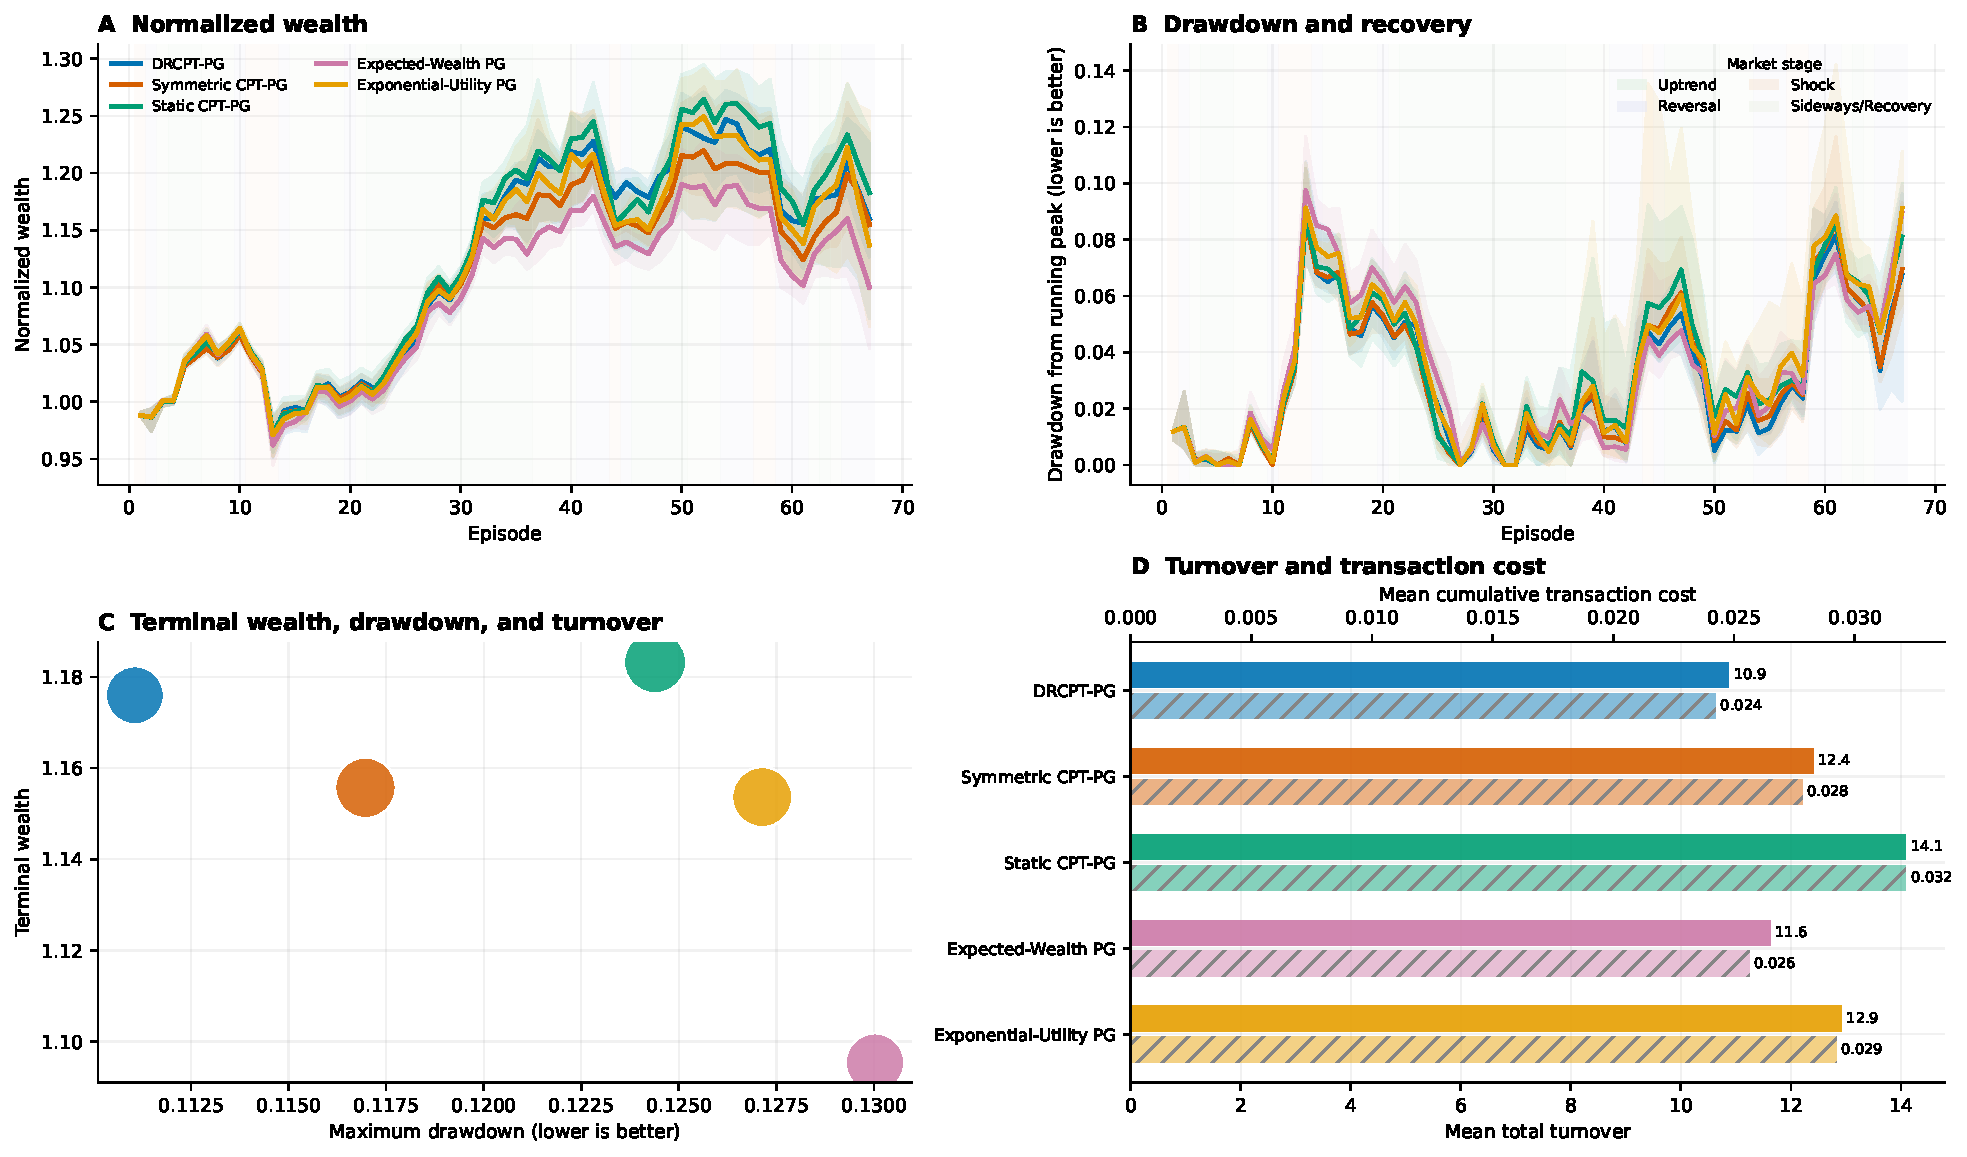
\includegraphics[width=\textwidth]{../../results/e5_hs300_e3sync_expcompatible_beta6_c10/figures/figure_E5_external_validity.pdf}
    \caption{E5 chronological A-share evaluation.  \textbf{A}: median normalized wealth across the ten policy seeds, with seed dispersion bands.  \textbf{B}: drawdown and recovery over the same replay, with market-stage annotations used only for visualization.  \textbf{C}: terminal wealth versus maximum drawdown; bubble size represents turnover.  \textbf{D}: mean turnover and cumulative transaction cost.  All learned methods share the same fixed asset universe, point-in-time information set, transaction-cost rule, and stochastic execution protocol.}
    \label{fig:e5-market}
\end{figure}

\begin{table}[t]
\centering
\small
\caption{E5 real-market summary.  Entries are means across the ten policy seeds; the equal-weight row is the deterministic passive anchor.}
\label{tab:e5-market}
\begin{tabular}{lrrrrr}
\toprule
Method & Ann. return (\%) & Sharpe & Max DD (\%) & Turnover & Cost (\%) \\
\midrule
DRCPT-PG & 13.03 & 0.856 & 11.67 & 10.87 & 2.42 \\
Symmetric CPT-PG & 13.21 & 0.796 & 12.48 & 12.41 & 2.78 \\
Static CPT-PG & 14.69 & 0.789 & 14.36 & 14.09 & 3.21 \\
Expected-Wealth PG & 10.51 & 0.606 & 14.23 & 11.63 & 2.56 \\
Exponential-Utility PG & 14.79 & 0.773 & 13.95 & 12.92 & 2.92 \\
Equal Weight & 16.64 & 1.068 & 11.59 & 1.00 & 0.20 \\
\bottomrule
\end{tabular}
\end{table}
\FloatBarrier

\paragraph{Results.}
Across the learned policies, DRCPT-PG occupies the strongest average risk-adjusted and trading-efficiency profile in the replay.  Its mean annualized return is $13.03\%$ with annualized volatility $15.62\%$, giving the highest learned-policy Sharpe ratio, $0.856$.  It also has the lowest learned-policy maximum drawdown, $11.67\%$, and the lowest total turnover, $10.87$, with cumulative transaction cost $2.42\%$ (\Cref{tab:e5-market}).  Static CPT-PG and exponential-utility PG realize higher mean gross returns but do so in a region with larger drawdown, turnover, and cost, which is visible in the return--risk--turnover panel of \Cref{fig:e5-market}.  The equal-weight portfolio is retained as a passive market anchor rather than a policy-gradient ablation.  Thus the real-market separation of DRCPT-PG is a risk-adjusted and trading-intensity result: the endogenous reference mechanism changes how the learned policy uses risk and turnover under chronological A-share data, not merely its terminal wealth.

\subsection{E6: Investor behavior prediction}\label{sec:e6}
\paragraph{Design.}
E6 asks whether the reference state used by the portfolio model carries incremental information about real investor decisions.  The sample contains $306{,}444$ held-stock rebalance opportunities, with $71{,}854$ observations in the final chronological test split.  The outcome is whether the investor decreases the stock's target weight at the next rebalance.  Four logistic specifications use exactly the same observations, outcome, controls, and train--validation--test dates; they differ only in the reference representation: no reference, static purchase cost, symmetric adaptation, or asymmetric adaptation with $(\eta_+,\eta_-)=(0.40,0.10)$.  Common controls include holding age, previous weight, price, prior investor reduction behavior, and lagged market, portfolio, and social aggregates.  Uncertainty is assessed by $200$ paired investor-cluster bootstrap draws.

The behavioral statistic is recomputed under each reference representation rather than fixing gain and loss states to the static purchase cost.  For the same realized decisions, we therefore report the reduction rate when the position is above its own reference, the reduction rate when it is below its own reference, and their difference.  This separates two questions: whether a reference representation improves held-out prediction and whether the gain/loss partition that it induces aligns with the observed disposition asymmetry.

\begin{figure}[t]
    \centering
    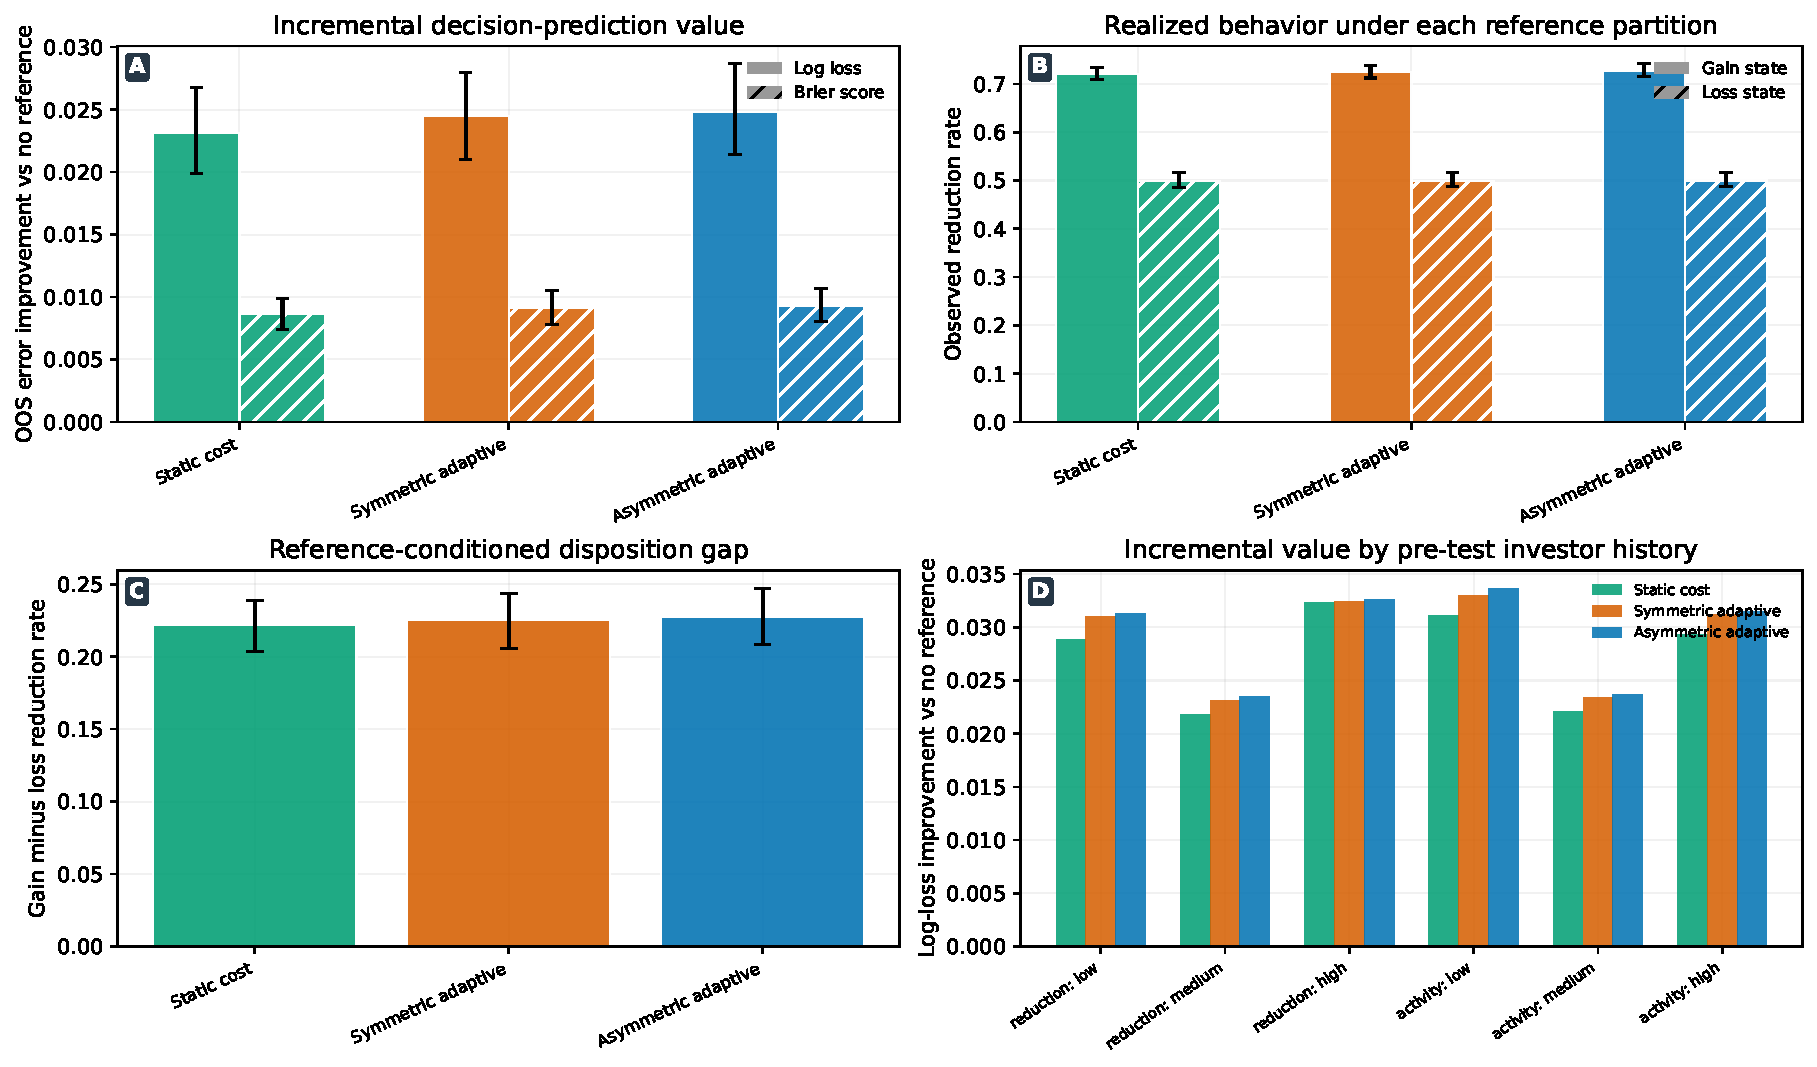
\includegraphics[width=\textwidth]{../../results/e6_reference_behavior_eta041/model/figures/figure_E6_behavior_alignment.pdf}
    \caption{E6 held-out behavioral alignment.  \textbf{A}: paired-bootstrap improvements in out-of-sample log loss and Brier score relative to the no-reference model.  \textbf{B}: observed reduction rates in gain and loss states defined separately by each reference.  \textbf{C}: reference-conditioned gain-minus-loss reduction gap.  \textbf{D}: log-loss improvement over the no-reference model across pre-test investor-history strata.  Error bars in A--C are paired investor-cluster 95\% bootstrap intervals.}
    \label{fig:e6-behavior}
\end{figure}
\FloatBarrier

\paragraph{Results.}
The asymmetric dynamic reference is the best of the four matched predictive specifications on every reported test metric.  On the $71{,}854$ held-out decisions it achieves log loss $0.57937$, Brier score $0.18696$, AUROC $0.78124$, and AUPRC $0.80909$, compared with $0.60420$, $0.19623$, $0.76002$, and $0.79060$ without a reference.  In the paired bootstrap, the asymmetric-minus-none difference is $-0.02488$ for log loss with 95\% interval $[-0.02866,-0.02142]$, $-0.00931$ for Brier score with interval $[-0.01070,-0.00803]$, $+0.02127$ for AUROC with interval $[0.01862,0.02394]$, and $+0.01852$ for AUPRC with interval $[0.01588,0.02126]$.

The comparison with symmetric adaptation isolates the value of gain--loss asymmetry beyond merely allowing the reference to move.  Relative to the symmetric reference, the asymmetric specification improves log loss by $0.000391$ (paired 95\% interval $[0.000014,0.000695]$ in the improvement direction) and AUROC by $0.000412$ (interval $[0.000164,0.000664]$).  Its reference-conditioned gain and loss reduction rates are $0.7278$ and $0.5004$, giving a disposition gap of $0.2274$; the paired-bootstrap gap is $0.2279$ with interval $[0.2085,0.2473]$.  The asymmetric gap exceeds the symmetric one by $0.00255$ with interval $[0.00107,0.00404]$.  The same specification also gives the largest log-loss improvement in all six strata formed from pre-test reduction history and trading activity (\Cref{fig:e6-behavior}D).  E6 therefore links the E1 reference mechanism to actual held-out decisions: asymmetric reference adaptation contributes stable incremental predictive information, while the estimand remains behavioral alignment rather than causal identification.

\subsection{E7: Simulated heterogeneous-investor interaction}\label{sec:e7}
\paragraph{Design.}
E7 adds an interaction layer without retraining the portfolio policies.  We calibrate four investor types from $3{,}481$ real users using training-period E6 gain/loss reduction statistics together with historical activity, diversification, sentiment, and network summaries.  The resulting population shares are $49.4\%$ moderate-frequency focused investors, $28.7\%$ disposition-effect investors, $19.4\%$ active diversified investors, and $2.5\%$ low-frequency diversified investors.  Sixteen calibrated users are sampled per type, producing $64$ simulated agents.  Type construction uses training-period behavioral summaries only; the global E6 predictive coefficients are not clustering features.

For every method, the experiment exactly replays the full cash-plus-300-stock recommendations saved by E5.  At the beginning of each five-day episode, adoption is sampled from the current recommendation, calibrated investor history, compatibility, and lagged satisfaction before any return from the episode is observed.  If the recommendation is adopted, the agent executes that method for five days; otherwise it keeps the episode-start portfolio.  Both paths apply their own trading costs and reference updates.  Conditional satisfaction is the five-day normalized prospect-value improvement over the no-rebalance counterfactual, and interaction value multiplies that satisfaction by adoption so that rejected recommendations contribute zero.  Seed-level market paths and adoption draws are paired across methods, and population summaries are weighted by the empirical type shares.

\begin{figure}[t]
    \centering
    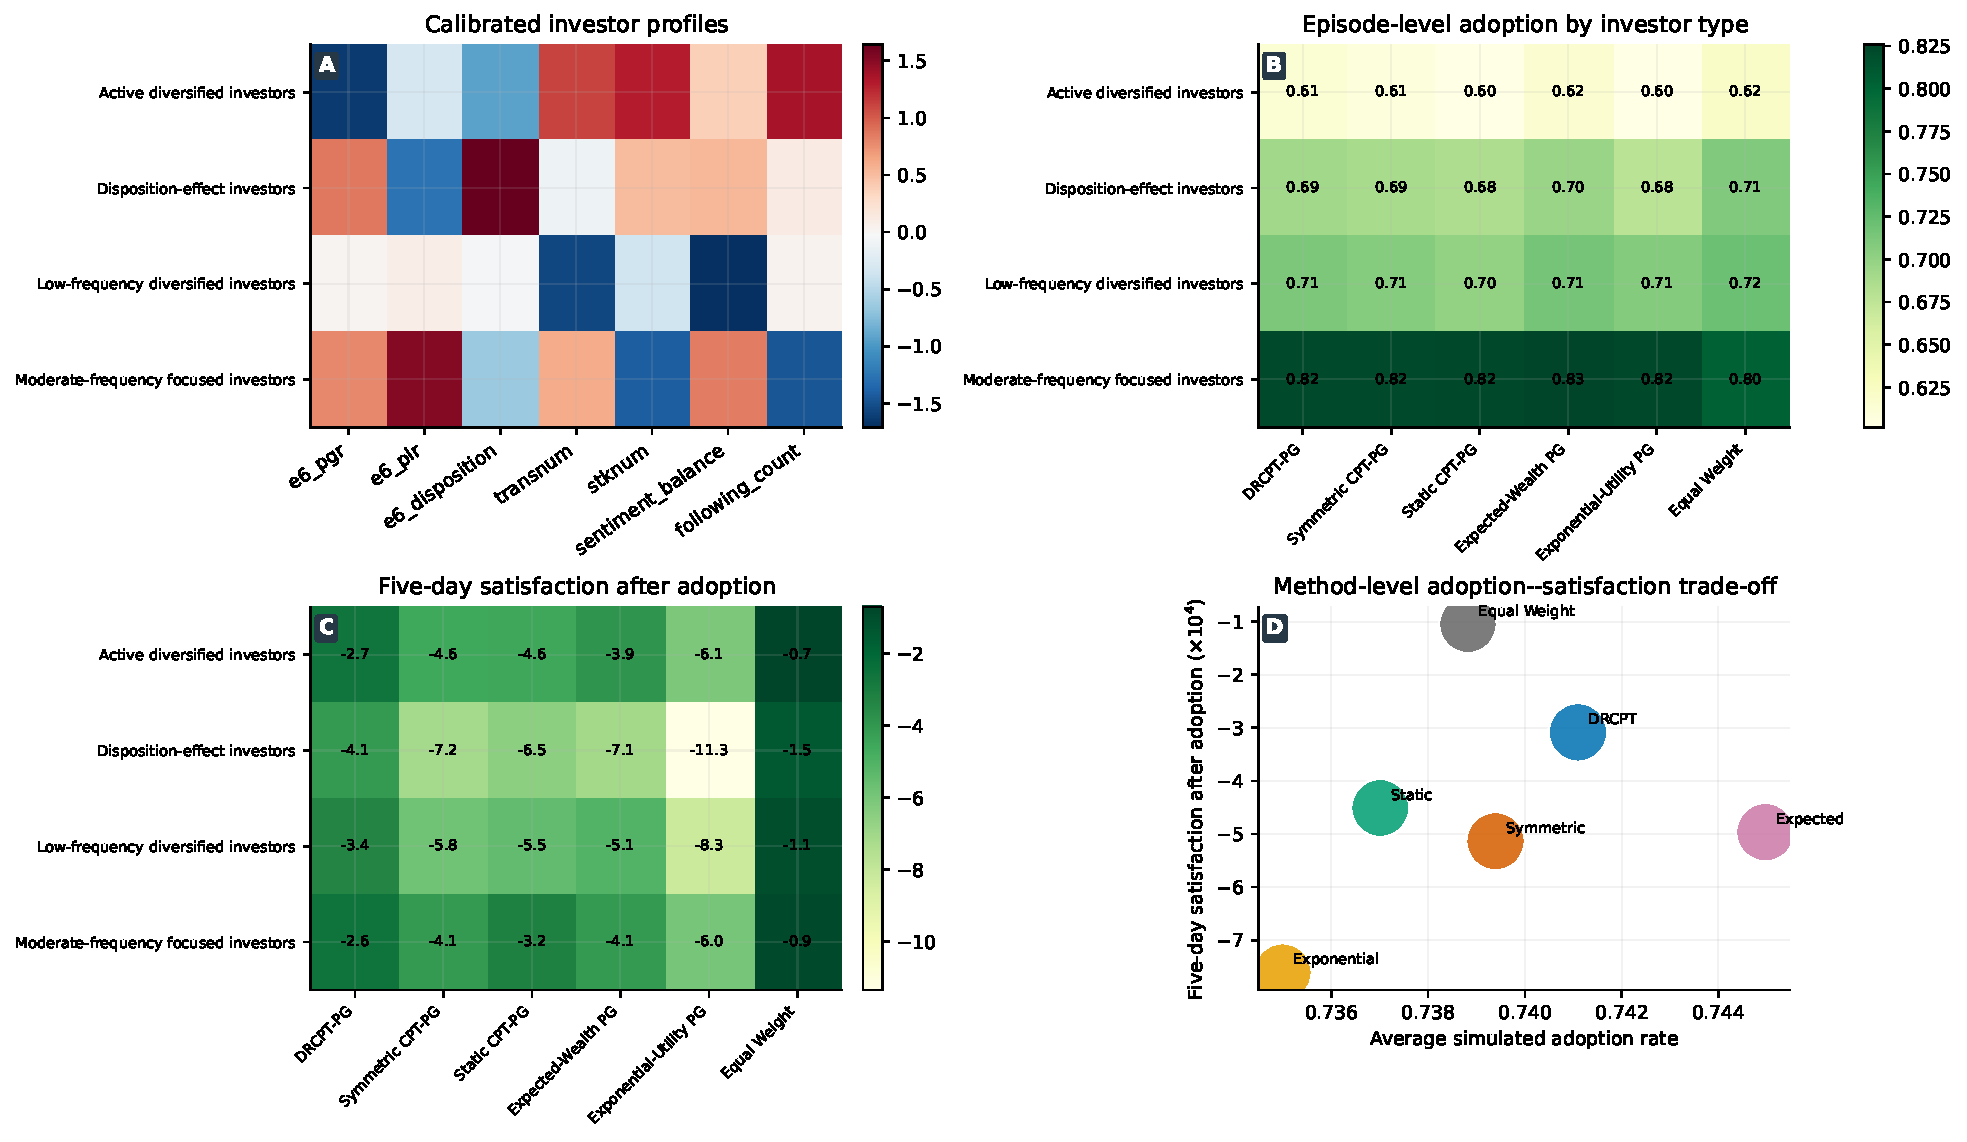
\includegraphics[width=\textwidth]{../../results/e7_heterogeneous_agents/figures/figure_E7_heterogeneous_agents.pdf}
    \caption{E7 calibrated heterogeneous-agent interaction.  \textbf{A}: standardized profiles of the four investor types.  \textbf{B}: simulated episode-level adoption by type and method.  \textbf{C}: five-day conditional satisfaction after adoption.  \textbf{D}: method-level adoption--satisfaction plane; bubble size encodes mean recommendation compatibility.  Adoption is decided before episode returns are revealed, and satisfaction is evaluated against a no-rebalance counterfactual with its own reference path.}
    \label{fig:e7-agents}
\end{figure}
\FloatBarrier

\paragraph{Results.}
The interaction layer separates recommendation uptake from value after uptake.  DRCPT-PG has a population-weighted adoption rate of $0.741$ and mean compatibility of $0.747$.  Its conditional five-day satisfaction is $-3.087\times10^{-4}$ and its adoption-weighted interaction value is $-2.265\times10^{-4}$.  Among the learned advisers, both are the largest values: the interaction values are $-3.237\times10^{-4}$ for static CPT-PG, $-3.739\times10^{-4}$ for symmetric CPT-PG, $-3.662\times10^{-4}$ for expected-wealth PG, and $-5.496\times10^{-4}$ for exponential-utility PG.  Expected-wealth PG has a slightly higher adoption rate ($0.745$) but lower post-adoption satisfaction, illustrating why adoption and satisfaction are kept as separate axes in \Cref{fig:e7-agents}D.

The learned-adviser ordering is also stable across heterogeneous types.  DRCPT-PG has the highest adoption-weighted interaction value among the learned methods for active diversified, disposition-effect, low-frequency diversified, and moderate-frequency focused investors, despite their different activity, diversification, and reference profiles.  It also uses lower mean turnover ($9.29$) and cumulative transaction cost ($0.0208$) than the other learned advisers in the interaction replay.  The passive equal-weight anchor is shown separately in the same figure; the E7 claim concerns relative behavior within the adaptive learned-adviser family.  Because adoption and satisfaction are calibrated counterfactual quantities, E7 is interpreted as a heterogeneity stress test of the recommendation layer, complementing the observed-decision evidence in E6.
